\chapter{Introduction}
Image analysis can be used in the diagnosis of diseases in different ways.
A lot of the data used for diagnosing come in the form of images.
Examples of these are MRI, CT, PET, ultrasound but also just plain images of body parts.
Understanding these images is often done using machine learning models in different forms.
In their nature, these models are not easy to understand and can therefore end up biased without
the model designer knowing it.

This project focuses on the HAM10000 dataset\cite{Tschandl_2018}, which contains images of skin lesions.
Doctors diagnose these lesions into different classes, some more dangerous than others.
The challenge on the HAM10000 dataset is to find a model that can predict the class of a given image.

\subsection{Biases in the data}
Many different models have been trained to diagnose lesions based on medical images.
These images are taken in a real world medical context, which can introduce unknown bias into the models.
It has even been reported that models trained on medical data where the lesions were masked out,
% THIS IS NOT TRUE! 73% percent refers to AUC not accuracy.
could reach an accuracy of $73\%$\cite{DeConstructing_Bias_on_Skin_Lesion_Datasets_2019}, indicating that there are other factors in the data, 
that can be used to classify the models than the actual lesion.
Some research has tried to introduce foreign object into the images,
and found that they changed the classification of the lesions \cite{Towards_Explainable_Classifiers_Using_the_Counterfactual_Approach_2019}.
These foreign objects included ruler markings, black frames and colored circles.

\section{The HAM10000 dataset}
The HAM10000 dataset contains 10015 images of skin lesions.
These images are a subset of the images from the ISIC dataset\cite{ISIC_Dataset_2018},
which collects images of skin lesions and hosts annual competitions for skin lesion diagnosis.
They are divided into seven classes as seen in the Table \ref{table:ham10000}.
A \textit{severity} has also been assigned each class.
These indicate if the lesion class benign, malignant or pre-malignant.
Malignant tumors are those where the cells are replicationg uncontrollably,
and there is a risk of these cells spreading to the rest of the body.
Beningn tumors can still hurt the patient, but are much less of a worry,
as they are not replicationg uncontrollably and hence do not lead to cancer.

\begin{table}[ht]
\begin{center}
\begin{tabular}{|c|c|c|c|c|c|c|}
\hline
Label    & Name                          & Severity      & Dataset prevalence \\ \hline
akiec    & Bowens disease                & pre-malignant & $3.27\%$           \\ \hline
nv       & Melanocytic nevi              & benign        & $66.94\%$          \\ \hline
mel      & Melanoma                      & malignant     & $11.11\%$          \\ \hline
bkl      & Benign keratosis-like lesions & benign        & $10.97\%$          \\ \hline
bcc      & Basal cell carcinoma          & malignant     & $5.13\%$           \\ \hline
vasc     & Vascular lesions              & benign        & $1.41\%$           \\ \hline
df       & Dermatofibroma                & benign        & $1.14\%$           \\ \hline
\end{tabular}
\end{center}

\caption{Overview of the HAM10000 dataset.}
\label{table:ham10000}
\end{table}

\subsection{State of the art models}\label{sec:state-of-the-art}
Due to the public nature of the dataset, many different models have been trained on it.
As of the time of writing, the best performing model published in a scientific paper,
reaches an accuracy of $93.4\%$\cite{datta2021soft}.

\subsection{Confounding elements in the data} \label{sec:confounding}
The dataset contains images of skin lesions, which are taken in a real world medical context.
In this context doctors might introduce foreign objects into the images,
to help in the treatment of the patient.
Examples of these can be seen on Figure \ref{fig:confounding_objects}.

\begin{figure}[ht]
    \begin{center}
        \begin{subfigure}[b]{0.3\textwidth}
            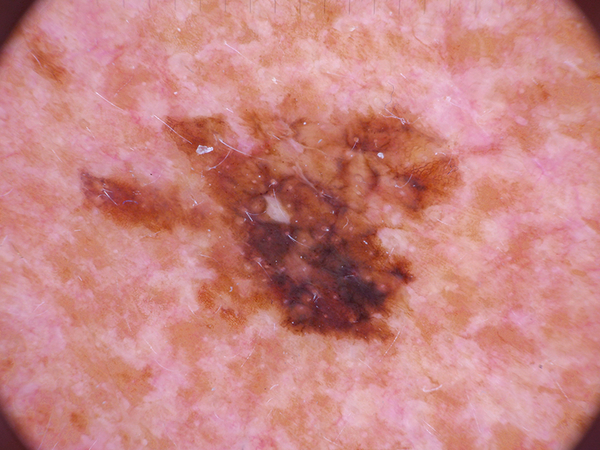
\includegraphics[width=\textwidth]{./images/ISIC_0024310.jpg}
            \caption{Image with black frame}
        \end{subfigure}
        \begin{subfigure}[b]{0.3\textwidth}
            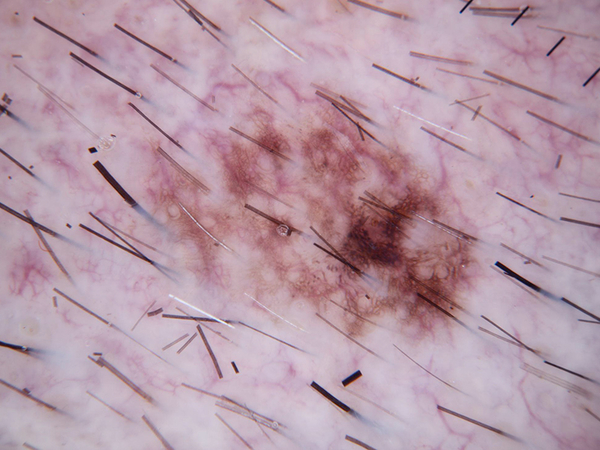
\includegraphics[width=\textwidth]{./images/ISIC_0024420.jpg}
            \caption{Image with ruler}
        \end{subfigure}
        \begin{subfigure}[b]{0.3\textwidth}
            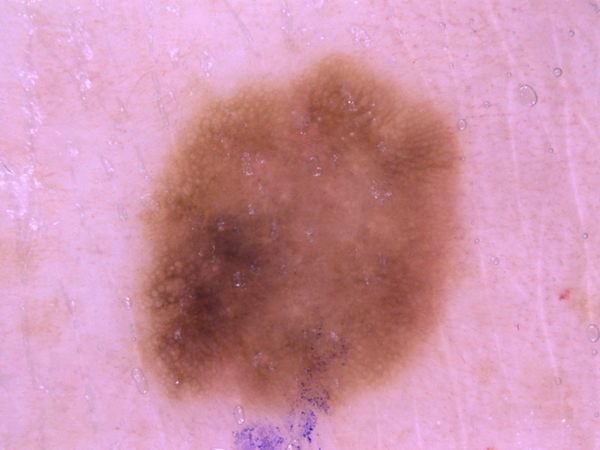
\includegraphics[width=\textwidth]{./images/ISIC_0027514.jpg}
            \caption{Image with blue ink}
        \end{subfigure}
    \end{center}
    \caption{Images with different confounding objects}
    \label{fig:confounding_objects}
\end{figure}

Labeling some of these confounding objects, we see that the rulers occur way more often than the others with a prevalence of roughly $17\%$ (See Table \ref{table:confounding_objects}).
Due to this higher prevalence, the study done in this project will focus on the ruler markings over the other confounding objects.

\begin{table}
    \centering
    \begin{tabular}{|l|r|}
        % confounding_objects.ipynb
        \hline 
        Confounder &  Prevalence \\ \hline
        ruler   &  0.171842 \\ \hline
        sticker &  0.000100 \\ \hline
        ink     &  0.003495 \\ \hline
    \end{tabular}
    \caption{Dataset prevalence of confounding objects}
    \label{table:confounding_objects}
\end{table}

\subsection{Correlation between confounding elements and HAM10000 labels}
On Figure \ref{fig:ruler_vs_dx} indications of correlations between the ruler markings and the HAM10000 labels can be seen.

\begin{figure}[ht]

\centering
\includegraphics[width=0.8\textwidth]{./build/confounder_label_correlation/confusion_matrix_seaborn.png}
\caption{Confusion matrix of rulers vs. class in the HAM10000 dataset - normalized over the x-axis.}
\label{fig:ruler_vs_dx}
\end{figure}

The two benign classes \textit{mel} and \textit{bkl} are both over represented on pictures with ruler markings copared to those without.
In general almost every class except the biggest \textit{nv} class is over represented.
The hypothesis that the presence of rulers in the images is correlated with the HAM10000, can be confirmed by a $\chi^2$-contingency test.
The null hypothesis of this test is that the presence of rulers in the images is not correlated with the HAM10000 labels.
The test value is 
    $\input{build/confounder_label_correlation/chi2.txt}$
on a test with
    $\input{build/confounder_label_correlation/dof.txt}$
degrees of freedom, resulting in a $p$-value of 
    $\input{build/confounder_label_correlation/p.txt}$
which is obviously significant.
